% ============================================================
%  FastAid — Final SRS 
% ============================================================
\documentclass[12pt,a4paper]{article}

% ── packages ──────────────────────────────────────────────
\usepackage[margin=1in]{geometry}
\usepackage{newtxtext,newtxmath}
\usepackage{graphicx}
\usepackage{booktabs}
\usepackage{tabularx}
\usepackage{longtable}
\usepackage{enumitem}
\usepackage{hyperref}
\usepackage[table]{xcolor}
\usepackage{fancyhdr}
\usepackage{titlesec}
\usepackage{tocloft}
\usepackage{float}
\usepackage{amsmath}
\usepackage{tikz}
\usetikzlibrary{shapes,arrows.meta,positioning,fit,backgrounds,calc}

% ── colours ───────────────────────────────────────────────
\definecolor{fastorange}{HTML}{0D47A1} % Maximum Deep Blue (Navy/Royal)
\definecolor{lightorange}{HTML}{E3F2FD} % Very pale icy blue background
\definecolor{darkgray}{HTML}{1A237E}   % Deep indigo-grey
\definecolor{medgray}{HTML}{455A64}    % Modern medium blue-grey
\definecolor{fastblue}{HTML}{00B0FF}   % Eye-catching Cyan-Blue
\definecolor{warnred}{HTML}{D50000}    % Sharp emergency red

% ── hyperlinks ────────────────────────────────────────────
\hypersetup{
    colorlinks=true,
    linkcolor=fastorange,
    urlcolor=fastblue,
    citecolor=fastorange
}

% ── header / footer ──────────────────────────────────────
\pagestyle{fancy}
\fancyhf{}
\fancyhead[L]{\small\textcolor{medgray}{Software Requirement Specification (SRS) For FastAid}}
\fancyfoot[C]{\thepage}
\renewcommand{\headrulewidth}{0.4pt}

% ── section styling ──────────────────────────────────────
\titleformat{\section}
  {\Large\bfseries\color{fastorange}}{\thesection}{1em}{}
\titleformat{\subsection}
  {\large\bfseries\color{darkgray}}{\thesubsection}{1em}{}
\titleformat{\subsubsection}
  {\normalsize\bfseries\color{medgray}}{\thesubsubsection}{1em}{}

% ── spacing ──────────────────────────────────────────────
\setlength{\parskip}{6pt}
\setlength{\parindent}{0pt}

% ── custom command for FR boxes ──────────────────────────
\newcommand{\frbox}[5]{%
  \begin{table}[H]
  \centering
  \begin{tabularx}{\textwidth}{|l|X|}
  \hline
  \rowcolor{lightorange}
  \textbf{Requirement ID} & \textbf{#1} \\
  \hline
  \textbf{Primary Actor} & #2 \\
  \hline
  \textbf{Trigger} & #3 \\
  \hline
  \textbf{Description} & #4 \\
  \hline
  \rowcolor{lightorange}
  \textbf{Acceptance Criteria} & #5 \\
  \hline
  \end{tabularx}
  \end{table}
}

% ══════════════════════════════════════════════════════════
\begin{document}

% ── title page ───────────────────────────────────────────
\begin{titlepage}
\centering
\vspace*{1.5cm}

{\Huge\bfseries\textcolor{fastorange}{FastAid}}\\[0.5cm]
{\Large A First Responder Volunteer Network with\\
Real-Time GPS Dispatch and AI Medical Analysis\\
for High-Density Urban Environments}

\vspace{1.5cm}

{\large\textbf{Software Requirements Specification}}\\[0.3cm]
{\normalsize Version 2.0 (Current Implementation) }

\vspace{2cm}

\begin{tabular}{rl}
\textbf{Submitted to:} & Md. Abu Sayed \\
                         \\[0.8cm]
\textbf{Prepared by:}  & Elora Sharmin Khan \\
                        & ID: 2231368 \\[0.8cm]
\textbf{Date:}         & \today
\end{tabular}

\vfill

\end{titlepage}

% ── table of contents ────────────────────────────────────
\newpage
\tableofcontents
\newpage

% ══════════════════════════════════════════════════════════
%  1. EXECUTIVE SUMMARY
% ══════════════════════════════════════════════════════════
\section{Executive Summary}

This is the Software Requirements Specification for FastAid. FastAid is an online, real-time emergency response platform that bridges the gap between emergency victims and trained first aid volunteer responders. The inspiration for FastAid originates from the frequent delays caused by heavy traffic and high dispatch latencies of traditional ambulance services in high-density urban environments. Often, critical life-saving interventions (such as CPR or hemorrhage control) fail to reach victims in time.

FastAid aims to change that. By initiating an emergency request from a mobile device, a victim automatically broadcasts their GPS location. FastAid instantly matches this with verified volunteers within a 5km radius. The system also leverages an AI engine to analyze the emergency description and provide an immediate severity grading and responder advice. 

The big-picture objectives are straightforward:
\begin{itemize}[leftmargin=2em]
  \item Offer victims an ultra-fast method to dispatch nearby medical help with automatic GPS capture.
  \item Track volunteer locations dynamically using WebSockets to ensure the closest responders are prioritized and visible to the victim.
  \item Leverage AI analysis to evaluate the emergency description and mentally prepare volunteers while en route.
  \item Maintain a secure administrative environment to verify medical credentials before volunteers go live.
\end{itemize}

% ══════════════════════════════════════════════════════════
%  2. INTRODUCTION
% ══════════════════════════════════════════════════════════
\section{Introduction}

FastAid is targeted at urban populations where ambulance arrival times frequently exceed 10-15 minutes. The system addresses this gap by crowdsourcing verified medical intervention. Our foundational research indicates that immediate first aid significantly increases survival rates in life-threatening scenarios.

\subsection{Purpose}
The purpose of this document is to explain how FastAid functions, how it is developed, and its system constraints. This encompasses functional requirements (what the system does), non-functional requirements (how well the system performs), and the architectural considerations. 

\subsection{Documents Conventions}
Features, headings, and key technical words are shown in bold.
\begin{itemize}[leftmargin=2em]
  \item Survey data and explanation of technical terms are shown in italics.
  \item Code is used to show the root path, database field names, and technical IDs (e.g. \texttt{/admin/users}, \texttt{lastKnownLocation}).
  \item Quotation marks display the text of labels and buttons (e.g. ``Start GPS sharing,'' ``Accept Case'').
\end{itemize}

\subsection{Who should read this and how}
The intended audience for this document is:
\begin{enumerate}[leftmargin=2em]
  \item Developers - as a robust reference during continuous development.
  \item Project Managers - to understand feature priorities and implementation logic.
  \item System Administrators - who oversee operations and need to understand the RBAC (Role-Based Access Control) mechanisms.
\end{enumerate}

\subsection{Problem Definition}
Citizens in urban environments suffer severely from high ambulance dispatch latencies. Research highlights that every minute of delay in critical medical emergencies drastically lowers the survival rate. The situation is exacerbated by:
\begin{enumerate}[leftmargin=2em]
  \item \textbf{Traffic Congestion}: Ambulances cannot bypass severe gridlock in peak urban hours.
  \item \textbf{Lack of Immediate Care}: Bystanders often panic and lack the confidence or training to intervene.
  \item \textbf{Information Asymmetry}: Even when help arrives, they often lack contextual knowledge of the victim's pre-existing conditions or the exact severity of the trauma.
\end{enumerate}
FastAid addresses these issues by leveraging a hyper-local network of community volunteers on foot or light vehicles, empowered with AI analysis of the crisis.

\subsection{Scope of Work}

\subsubsection*{In-Scope}
\begin{enumerate}[leftmargin=2em]
  \item User authentication and Role-Based Access Control (Victim, Volunteer, Admin).
  \item Emergency Requesting: Auto-GPS detection, description capture, and photo upload.
  \item AI Integration: Automated evaluation of severity, key injuries, and medical advice via an LLM service.
  \item Real-Time Tracking: Socket.IO driven volunteer location broadcasting.
  \item Notification Engine: Web-Push notifications with SMS fallbacks for guaranteed delivery.
  \item Admin Dashboard: Credential verification, log viewing, and system metrics.
\end{enumerate}

\subsubsection*{Out-of-Scope}
\begin{enumerate}[leftmargin=2em]
  \item Full ambulance dispatch system integration (system focuses only on crowdsourced volunteers).
  \item Post-emergency User Rating \& Feedback systems (removed to lower user friction during distress).
  \item Long-term medical record storage beyond basic allergies and blood type profiles.
\end{enumerate}

\subsection{Overview}
FastAid is a Node.js/Express web application utilizing a real-time, event-driven architecture. It features a responsive mobile-first UI for victims and volunteers, an Express backend serving REST APIs, a Socket.IO server for GPS tracking, an AI engine for text analysis, and a MongoDB database with Mongoose ORM utilizing \texttt{2dsphere} geospatial indexing.

\subsection{Technical specifications}
\label{sec:techspec}

\subsubsection*{Frontend}
\begin{itemize}[leftmargin=2em]
  \item Mobile-first stress-friendly interfaces designed to be accessed under panic.
  \item No heavy frameworks; relies on vanilla HTML5/JS for the client apps (\texttt{victim-mobile}, \texttt{volunteer-phone}).
  \item Leaflet maps with OpenStreetMap tiles for rendering realtime location data efficiently.
\end{itemize}

\subsubsection*{Backend}
\begin{itemize}[leftmargin=2em]
  \item Node.js with Express.js routing.
  \item Custom RBAC (Role-Based Access Control) middleware.
  \item Realtime WebSockets managed via Socket.IO.
  \item Web-Push API and SMS fallbacks for sub-3-second notification delivery.
\end{itemize}

\subsubsection*{Database}
\begin{itemize}[leftmargin=2em]
  \item MongoDB with Mongoose ORM.
  \item Geospatial queries enabled via \texttt{2dsphere} indexing on \texttt{lastKnownLocation}.
  \item Atomic transactions applied to responder acceptance to prevent duplicate dispatching.
\end{itemize}

\subsubsection*{AI Engine}
\begin{itemize}[leftmargin=2em]
  \item Integration with an external LLM Service (\texttt{services/llm.service.js}).
  \item Automatically parses raw emergency descriptions to output structured JSON: severity, key injuries, victim advice, and responder advice.
\end{itemize}

% ── System Architecture Diagram ──────────────────────────
\subsection{System Architecture Diagram}

Figure~\ref{fig:arch} demonstrates the decoupled, real-time architecture of FastAid.

\begin{figure}[H]
\centering
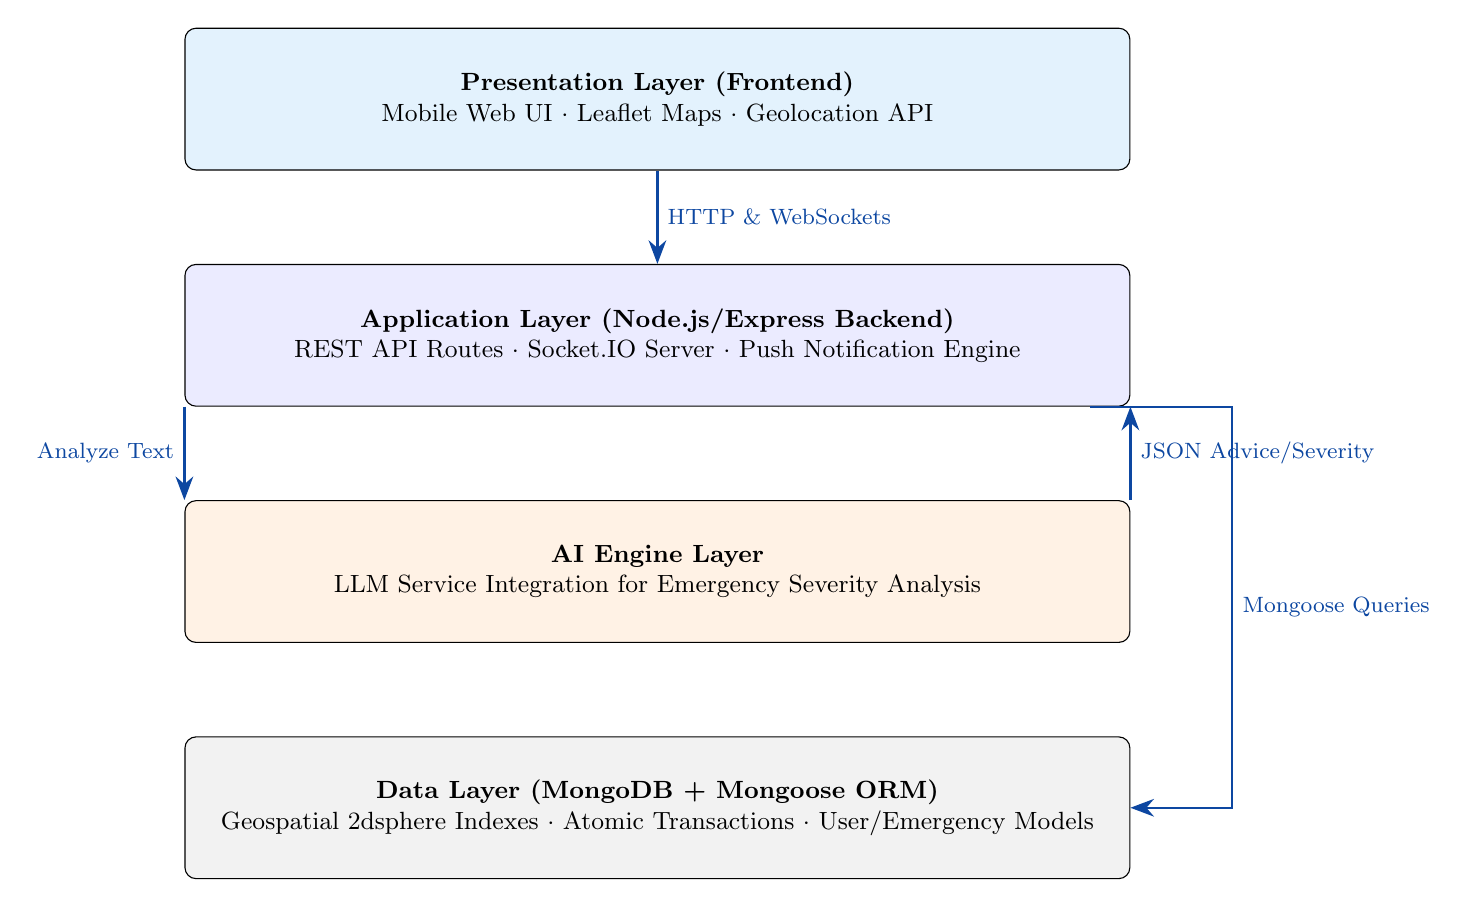
\begin{tikzpicture}[
    layer/.style={draw, rounded corners, minimum width=12cm,
                  minimum height=1.8cm, align=center, font=\small},
    arrow/.style={-{Stealth[length=3mm]}, thick, color=fastorange},
    label/.style={font=\footnotesize\color{medgray}}
]
% --- layers ---
\node[layer, fill=lightorange]               (fe) at (0,0)
  {\textbf{Presentation Layer (Frontend)}\\
   Mobile Web UI $\cdot$ Leaflet Maps $\cdot$ Geolocation API};

\node[layer, fill=blue!8]                   (be) at (0,-3)
  {\textbf{Application Layer (Node.js/Express Backend)}\\
   REST API Routes $\cdot$ Socket.IO Server $\cdot$ Push Notification Engine};

\node[layer, fill=orange!10]                (ai) at (0,-6)
  {\textbf{AI Engine Layer}\\
   LLM Service Integration for Emergency Severity Analysis};

\node[layer, fill=gray!10]                  (db) at (0,-9)
  {\textbf{Data Layer (MongoDB + Mongoose ORM)}\\
   Geospatial 2dsphere Indexes $\cdot$ Atomic Transactions $\cdot$ User/Emergency Models};

% --- arrows ---
\draw[arrow] (fe.south) -- node[right, label]{HTTP \& WebSockets} (be.north);
\draw[arrow] (be.south west) -- node[left, label]{Analyze Text} (ai.north west);
\draw[arrow] (ai.north east) -- node[right, label]{JSON Advice/Severity} (be.south east);
\draw[arrow] ([xshift=5.5cm]be.south) -- ++(1.8,0) |- node[near start, right, label]{Mongoose Queries} (db.east);

\end{tikzpicture}
\caption{FastAid System Architecture (Four-Layer Design)}
\label{fig:arch}
\end{figure}

\subsection{User Interface}
The user interface avoids heavy single-page application overhead, instead relying on separated web directories optimized for specific roles:
\begin{itemize}[leftmargin=2em]
  \item \textbf{Victim Mobile}: Features massive, high-contrast buttons intended for use during a panic response. A prominent Leaflet map dynamically tracks the assigned volunteer.
  \item \textbf{Volunteer Phone}: Focused on a continuous "Start GPS Sharing" toggle to maintain the WebSocket connection alive while running in the background.
  \item \textbf{Admin Dashboard}: A desktop-oriented table view for verifying uploaded medical certifications and assessing overall system metrics (latency, active emergencies).
\end{itemize}

\subsection{Hardware Interface}
FastAid requires no specialized hardware beyond standard smartphones equipped with a GPS module. The browser requires HTML5 Geolocation API permissions.

\subsection{Software Interface}
\begin{itemize}[leftmargin=2em]
  \item \textbf{Database Interfacing}: Mongoose translates Express payloads into strict schemas (\texttt{User}, \texttt{VolunteerProfile}, \texttt{Emergency}).
  \item \textbf{Maps API}: Leaflet interfaces with free OpenStreetMap tiles, avoiding costly proprietary map layers.
  \item \textbf{Push Notifications}: Service Workers interface with the \texttt{web-push} VAPID standard.
\end{itemize}

\subsection{Survey (5 First Responders / Victims)}
\begin{itemize}[nosep]
    \item \textbf{Locations:} High-density urban zones.
    \item \textbf{Key Findings:} 80\% of victims report ambulance wait times exceeding 15 minutes. 100\% of surveyed medical volunteers expressed willingness to respond to hyperlocal emergencies if alerted.
    \item \textbf{Critical Insight (``Preparedness Gap''):} Volunteers stated they often hesitate to rush into an emergency blindly. They require immediate context on the severity and nature of the injury to bring the correct first-aid kit.
\end{itemize}

\subsection{Document Analysis (10 Academic Papers)}
Papers analyzed across three themes:
\begin{enumerate}[nosep]
    \item \textbf{Crowdsourced Emergency Response} (4 papers) --- Validation that proximity-based volunteer dispatch outperforms centralized ambulance depots in dense cities \cite{zijlko2021, lee2022, smith2020}. Studies emphasize that optimizing phased alerting and predicting volunteer acceptance reduces operational latency \cite{lee2022}.
    \item \textbf{Trauma Survival Rates} (3 papers) --- Demonstrates the critical "Golden Hour" in trauma \cite{lerner2001} and how immediate bystander CPR drastically reduces mortality in out-of-hospital cardiac arrests \cite{hasselqvist2015, drennan2014}.
    \item \textbf{Mobile WebSockets \& GPS} (3 papers) --- Highlights the battery-efficiency of Socket.IO polling over traditional HTTP polling for tracking, and the need to optimize native location APIs to avoid draining responder phones \cite{pimentel2019, koutsonikola2015, zhang2020}.
\end{enumerate}

% ══════════════════════════════════════════════════════════
%  3. ELICITATION RESULTS
% ══════════════════════════════════════════════════════════
\section{Elicitation Results}

\subsection{Survey Results}
\textbf{Demographics:} 5 respondents including off-duty paramedics, nurses, and previous victims of traffic accidents. 

\begin{table}[h!]
\centering
\small
\begin{tabularx}{\textwidth}{|l|c|X|}
\hline
\rowcolor{lightorange}
\textbf{Finding} & \textbf{Value} & \textbf{Insight} \\
\hline
Ambulance Delay ($>15$ mins) & 80\% & Centralized dispatch is failing in traffic-heavy regions. \\
\hline
Willingness to volunteer & 100\% & High community willingness to intervene if properly notified. \\
\hline
Need for injury context & 100\% & Volunteers demand an understanding of the crisis prior to arriving. \\
\hline
Flaky internet connections & 60\% & Relies on SMS fallbacks when 4G data drops. \\
\hline
\end{tabularx}
\caption{Key survey findings}
\end{table}

\textbf{Key Insight --- ``Preparedness Gap'':} The data clearly shows that while volunteers are willing to help, they will not run blindly into an unknown situation. FastAid must act as an intelligent dispatcher, utilizing AI to summarize the panic-typed messages of a victim into actionable medical context for the responder.

\subsection{Document Analysis Results}
Research strongly supports the implementation of crowdsourced response. Studies show that systems utilizing strict 5km geolocation matching combined with atomic transaction assignments prevent "bystander effect" and "double-booking" of the same emergency.

% ══════════════════════════════════════════════════════════
%  4. LATEST FEATURES FROM FIELDWORK
% ══════════════════════════════════════════════════════════
\section{Latest Features from Fieldwork}

Based on the elicitation responses, the following critical features were baked into the FastAid platform:

\begin{longtable}{|c|p{4.5cm}|p{9.5cm}|}
\caption{Features derived from fieldwork with detailed user needs} \\
\hline
\rowcolor{lightorange}
\textbf{\#} & \textbf{Feature} & \textbf{User Need (from Survey)} \\
\hline
\endfirsthead
\hline
\rowcolor{lightorange}
\textbf{\#} & \textbf{Feature} & \textbf{User Need (from Survey)} \\
\hline
\endhead

F1 & Auto-GPS Request Capture & Victims under extreme stress cannot type an address accurately. Pressing one button to fetch HTML5 Geolocation is mandatory. \\
\hline
F2 & AI Emergency Analysis & Volunteers need to know if the victim is bleeding, unconscious, or burned. The LLM translates frantic descriptions into medical severity codes and advice. \\
\hline
F3 & Web-Push with SMS Fallback & Urban dead-zones drop data packets. If a Web-Push fails after 2000ms, the system must trigger a reliable SMS fallback to ensure the volunteer is notified. \\
\hline
F4 & Live Socket.IO Tracking & Victims experience extreme anxiety waiting for help. Watching the volunteer's GPS dot move on the Leaflet map in real-time provides immense psychological relief. \\
\hline
F5 & Medical Profiles & Responders need to know if the victim has pre-existing conditions (e.g., Asthma, Hemophilia) or specific blood types before administering care. \\
\hline
\end{longtable}

% ══════════════════════════════════════════════════════════
%  5. FEATURE COMPARISON: LITERATURE VS. FIELDWORK
% ══════════════════════════════════════════════════════════
\section{Feature Comparison: Literature vs. Fieldwork}

\begin{longtable}{|p{3.5cm}|p{3.5cm}|p{3.5cm}|p{4.5cm}|}
\caption{Old SRS vs.\ Current Implementation comparison} \\
\hline
\rowcolor{lightorange}
\textbf{Feature} & \textbf{Literature / Old SRS} & \textbf{Current Implementation} & \textbf{Analysis} \\
\hline
\endfirsthead
\hline
\rowcolor{lightorange}
\textbf{Feature} & \textbf{Literature / Old SRS} & \textbf{Current Implementation} & \textbf{Analysis} \\
\hline
\endhead

Proximity Dispatching & \checkmark & \checkmark & Core feature validated by both sources (5km matching). \\
\hline
Feedback \& Rating & \checkmark & -- & Fieldwork showed victims rarely review volunteers post-trauma; it adds unnecessary database friction and was removed. \\
\hline
Basic Text Requests & \checkmark & AI Analysis & Volunteers demanded structured actionable medical summaries rather than raw frantic text. \\
\hline
Static API Tracking & \checkmark & WebSockets & Users requested smooth, real-time map movement without polling delays. \\
\hline
\end{longtable}

% ══════════════════════════════════════════════════════════
%  6. SPECIFIC REQUIREMENTS
% ══════════════════════════════════════════════════════════
\section{Specific Requirements}

% ── Use Case Diagram ─────────────────────────────────────
\subsection{Use Case Diagram}

Figure~\ref{fig:usecase} gives an overview of the interactions between the three primary roles and the system.

\begin{figure}[H]
\centering
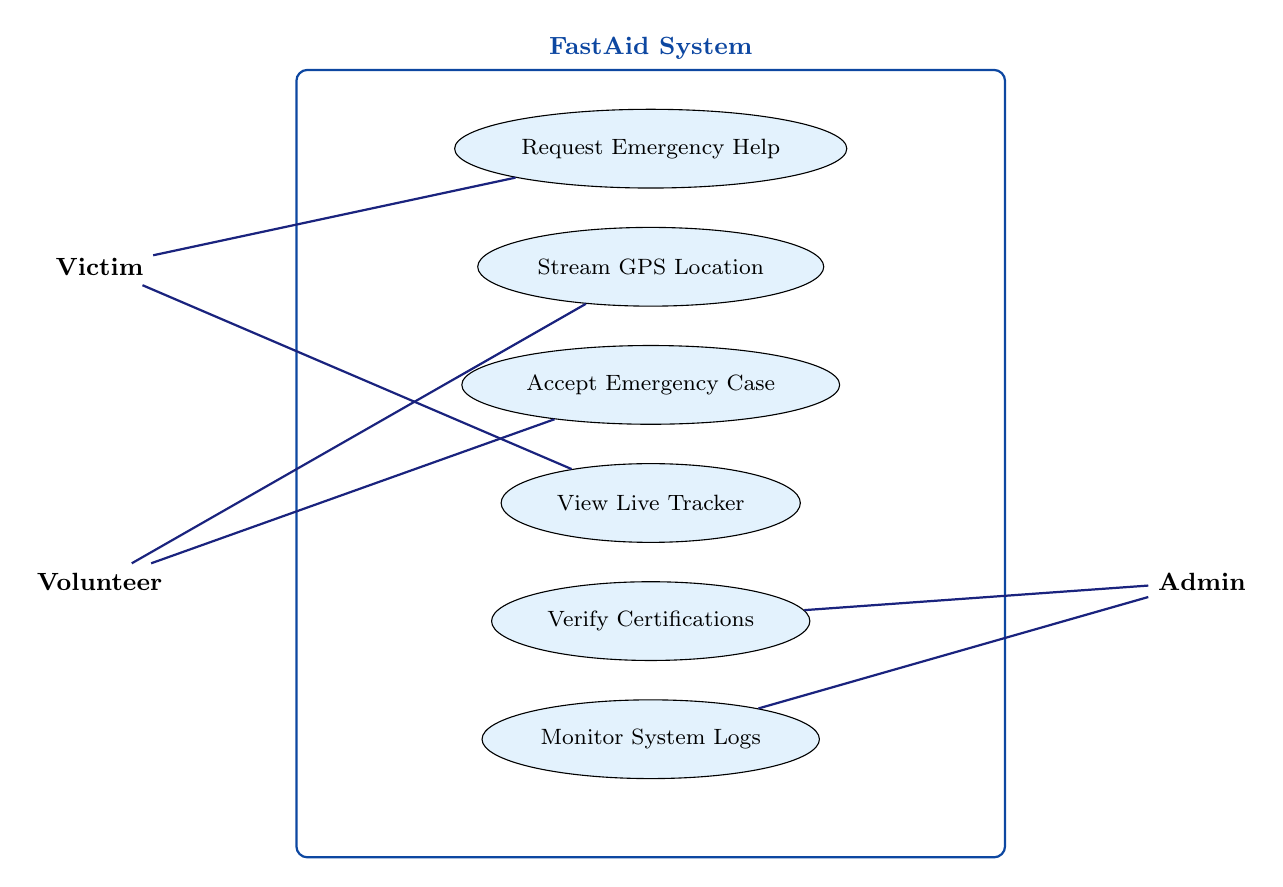
\begin{tikzpicture}[
    actor/.style={font=\small\bfseries},
    usecase/.style={draw, ellipse, minimum width=3.8cm, minimum height=1cm,
                    align=center, font=\footnotesize, fill=lightorange},
    sysbox/.style={draw=fastorange, thick, rounded corners, inner sep=12pt},
    conn/.style={-, thick, color=darkgray}
]

% --- system boundary ---
\node[sysbox, minimum width=9cm, minimum height=10cm, label={[font=\small\bfseries\color{fastorange}]above:FastAid System}] (sys) at (5.5,-5.5) {};

% --- use cases ---
\node[usecase] (uc1) at (5.5, -1.5) {Request Emergency Help};
\node[usecase] (uc2) at (5.5, -3.0) {Stream GPS Location};
\node[usecase] (uc3) at (5.5, -4.5) {Accept Emergency Case};
\node[usecase] (uc4) at (5.5, -6.0) {View Live Tracker};
\node[usecase] (uc5) at (5.5, -7.5) {Verify Certifications};
\node[usecase] (uc6) at (5.5, -9.0) {Monitor System Logs};

% --- actors (left: Victim / Volunteer) ---
\node[actor] (victim) at (-1.5, -3.0) {Victim};
\node[actor] (volunteer) at (-1.5, -7.0) {Volunteer};

% --- actors (right: Admin) ---
\node[actor] (admin)      at (12.5, -7.0) {Admin};

% --- connections: victim ---
\draw[conn] (victim) -- (uc1);
\draw[conn] (victim) -- (uc4);

% --- connections: volunteer ---
\draw[conn] (volunteer) -- (uc2);
\draw[conn] (volunteer) -- (uc3);

% --- connections: admin ---
\draw[conn] (admin) -- (uc5);
\draw[conn] (admin) -- (uc6);

\end{tikzpicture}
\caption{Use Case Diagram FastAid Actor Interactions}
\label{fig:usecase}
\end{figure}

% ── Sequence Diagram ─────────────────────────────────────
\subsection{Sequence Diagram --- Emergency Dispatch Flow}

Figure~\ref{fig:sequence} maps out the process of an emergency request being analyzed, dispatched, and accepted by a volunteer.

\begin{figure}[H]
\centering
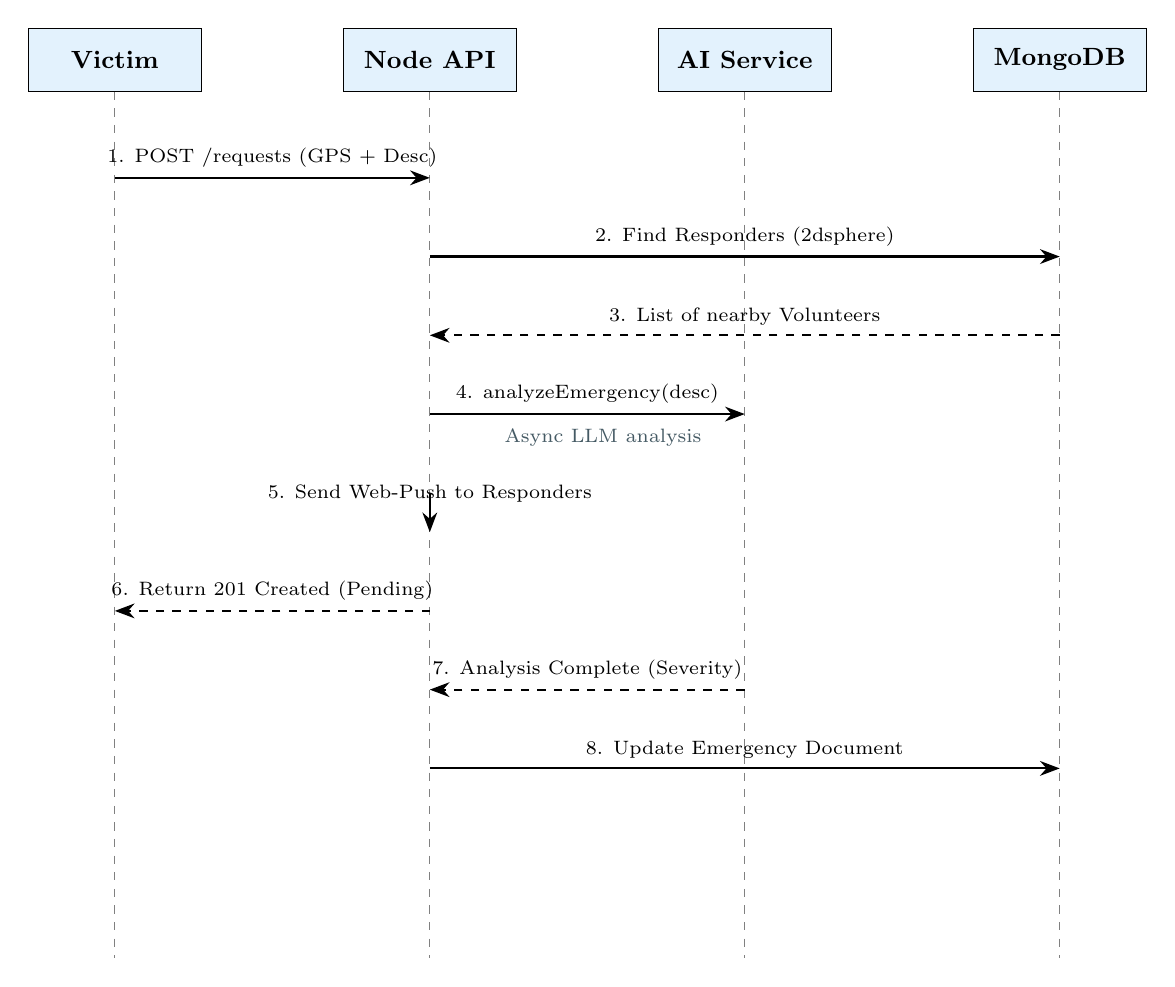
\begin{tikzpicture}[
    entity/.style={draw, rectangle, minimum width=2.2cm, minimum height=0.8cm,
                   fill=lightorange, font=\small\bfseries, align=center},
    msg/.style={-{Stealth[length=2.5mm]}, thick},
    rmsg/.style={-{Stealth[length=2.5mm]}, thick, dashed},
    note/.style={font=\scriptsize, align=left, color=medgray}
]

% --- entities ---
\node[entity] (user) at (0,0)   {Victim};
\node[entity] (flask) at (4,0)  {Node API};
\node[entity] (ai) at (8,0)     {AI Service};
\node[entity] (db) at (12,0)    {MongoDB};

% --- lifelines ---
\draw[dashed, gray] (user.south)  -- ++(0,-11);
\draw[dashed, gray] (flask.south) -- ++(0,-11);
\draw[dashed, gray] (ai.south)    -- ++(0,-11);
\draw[dashed, gray] (db.south)    -- ++(0,-11);

% --- messages ---
\draw[msg] (0,-1.5) -- node[above, font=\scriptsize]{1. POST /requests (GPS + Desc)} (4,-1.5);

\draw[msg] (4,-2.5) -- node[above, font=\scriptsize]{2. Find Responders (2dsphere)} (12,-2.5);

\draw[rmsg] (12,-3.5) -- node[above, font=\scriptsize]{3. List of nearby Volunteers} (4,-3.5);

\draw[msg] (4,-4.5) -- node[above, font=\scriptsize]{4. analyzeEmergency(desc)} (8,-4.5);
\node[note] at (6.2,-4.8) {Async LLM analysis};

\draw[msg] (4,-5.5) -- node[above, font=\scriptsize]{5. Send Web-Push to Responders} (4,-6.0);

\draw[rmsg] (4,-7.0) -- node[above, font=\scriptsize]{6. Return 201 Created (Pending)} (0,-7.0);

\draw[rmsg] (8,-8.0) -- node[above, font=\scriptsize]{7. Analysis Complete (Severity)} (4,-8.0);

\draw[msg] (4,-9.0) -- node[above, font=\scriptsize]{8. Update Emergency Document} (12,-9.0);

\end{tikzpicture}
\caption{Sequence Diagram from Request to AI Analysis}
\label{fig:sequence}
\end{figure}

% ── Activity Diagram ─────────────────────────────────────
\subsection{Activity Diagram --- Emergency Dispatch Lifecycle}

Figure~\ref{fig:activity} illustrates the complete lifecycle of an emergency from creation through to closure, including the AI analysis branch and the notification fallback mechanism.

\begin{figure}[H]
\centering
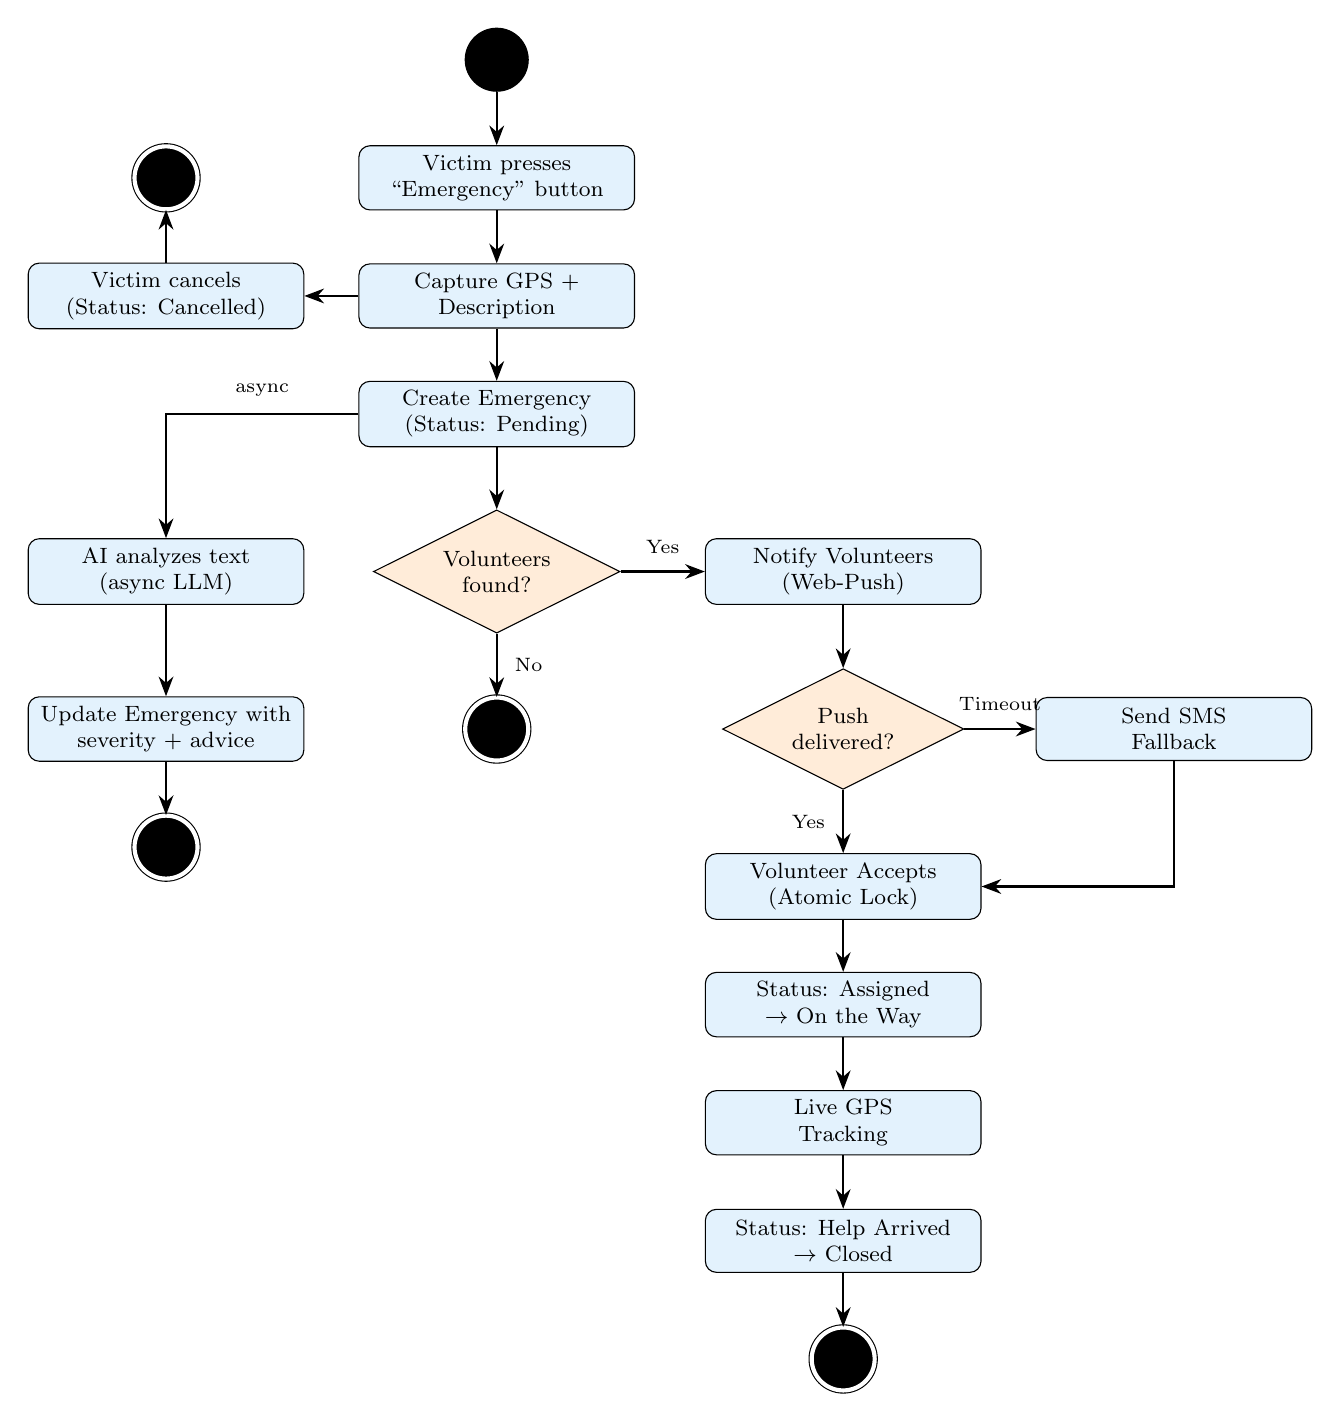
\begin{tikzpicture}[
    start/.style={circle, draw, fill=black, minimum size=8mm},
    stop/.style={circle, draw, fill=black, minimum size=8mm, double, double distance=1.5pt},
    activity/.style={draw, rounded corners=4pt, minimum width=3.5cm, minimum height=0.8cm,
                     align=center, font=\footnotesize, fill=lightorange},
    decision/.style={draw, diamond, aspect=2, minimum width=2cm, align=center,
                     font=\footnotesize, fill=orange!15},
    arrow/.style={-{Stealth[length=2.5mm]}, thick},
    note/.style={font=\scriptsize\itshape, color=medgray}
]

% --- nodes ---
\node[start] (s) at (0,0) {};

\node[activity] (a1) at (0,-1.5) {Victim presses\\``Emergency'' button};
\node[activity] (a2) at (0,-3.0) {Capture GPS +\\Description};
\node[activity] (a3) at (0,-4.5) {Create Emergency\\(Status: Pending)};

\node[decision] (d1) at (0,-6.5) {Volunteers\\found?};
\node[stop] (e_nomatch) at (0,-8.5) {};

\node[activity] (a4) at (4.4,-6.5) {Notify Volunteers\\(Web-Push)};
\node[decision] (d2) at (4.4,-8.5) {Push\\delivered?};
\node[activity] (a5) at (8.6,-8.5) {Send SMS\\Fallback};

\node[activity] (a6) at (4.4,-10.5) {Volunteer Accepts\\(Atomic Lock)};
\node[activity] (a7) at (4.4,-12.0) {Status: Assigned\\$\rightarrow$ On the Way};
\node[activity] (a8) at (4.4,-13.5) {Live GPS\\Tracking};
\node[activity] (a9) at (4.4,-15.0) {Status: Help Arrived\\$\rightarrow$ Closed};
\node[stop] (e) at (4.4,-16.5) {};

% --- AI async branch ---
\node[activity] (ai) at (-4.2,-6.5) {AI analyzes text\\(async LLM)};
\node[activity] (ai2) at (-4.2,-8.5) {Update Emergency with\\severity + advice};
\node[stop] (e_ai) at (-4.2,-10.0) {};

% --- cancel branch ---
\node[activity] (cancel) at (-4.2,-3.0) {Victim cancels\\(Status: Cancelled)};
\node[stop] (e_cancel) at (-4.2,-1.5) {};

% --- arrows ---
\draw[arrow] (s) -- (a1);
\draw[arrow] (a1) -- (a2);
\draw[arrow] (a2) -- (a3);
\draw[arrow] (a3) -- (d1);

\draw[arrow] (d1) -- node[above, font=\scriptsize, yshift=1mm]{Yes} (a4);
\draw[arrow] (d1) -- node[right, font=\scriptsize, xshift=1mm]{No} (e_nomatch);

\draw[arrow] (a4) -- (d2);
\draw[arrow] (d2) -- node[above, font=\scriptsize, yshift=1mm]{Timeout} (a5);
\draw[arrow] (d2) -- node[left, font=\scriptsize, xshift=-1mm]{Yes} (a6);
\draw[arrow] (a5) |- (a6);
\draw[arrow] (a6) -- (a7);
\draw[arrow] (a7) -- (a8);
\draw[arrow] (a8) -- (a9);
\draw[arrow] (a9) -- (e);

% --- AI async branch ---
\draw[arrow] (a3.west) -| node[near start, above, font=\scriptsize, yshift=1mm]{async} (ai.north);
\draw[arrow] (ai) -- (ai2);
\draw[arrow] (ai2) -- (e_ai);

% --- cancel branch ---
\draw[arrow] (a2.west) -- (cancel.east);
\draw[arrow] (cancel.north) -- (e_cancel.south);

\end{tikzpicture}
\caption{Activity Diagram --- Emergency Dispatch Lifecycle}
\label{fig:activity}
\end{figure}



% ── Component 1 ──────────────────────────────────────────
\subsection{Component 1: Victim \& Volunteer Registration and Authentication}

\subsubsection*{User Stories}
\begin{enumerate}[leftmargin=2em]
  \item A victim wants to register via mobile/email securely and store their medical profile (allergies, blood type) so responders are informed during a crisis.
  \item A volunteer wants to upload their medical certifications and toggle their availability status when they are off-duty.
\end{enumerate}

\subsubsection*{Functional Requirements}


\frbox{FR-02: Medical Profile Management}
{Victims}
{User accesses profile settings.}
{The user can populate the \texttt{medicalProfile} embedded document: \texttt{bloodType}, \texttt{allergies}, \texttt{preExistingConditions}, \texttt{emergencyContactName}, and \texttt{emergencyContactPhone}.}
{%
\begin{itemize}[leftmargin=1.5em]
  \item Updates immediately reflect in any future emergency dispatches.
  \item The emergency contact fields allow responders to notify a family member.
\end{itemize}
}

\frbox{FR-03: Volunteer Availability Toggle}
{Volunteers}
{Volunteer presses the "Go Offline/Online" button.}
{The \texttt{isAvailable} boolean on their \texttt{VolunteerProfile} is updated.}
{%
\begin{itemize}[leftmargin=1.5em]
  \item Offline volunteers must be entirely excluded from the \texttt{\$geoNear} MongoDB query during emergency matches.
\end{itemize}
}

\frbox{FR-04: Role-Based Access Control (RBAC)}
{All Users}
{User attempts to access a protected route (e.g., \texttt{/api/admin/system-logs}).}
{The custom RBAC middleware validates the user's role against the required route authorization.}
{%
\begin{itemize}[leftmargin=1.5em]
  \item Standard users receive HTTP 403 Forbidden on admin routes.
  \item Demo auth headers (\texttt{x-demo-role}) are utilized for testing environments.
\end{itemize}
}

% ── Component 2 ──────────────────────────────────────────
\subsection{Component 2: Emergency Request and AI Diagnosis}

\subsubsection*{User Stories}
\begin{enumerate}[leftmargin=2em]
  \item A victim wants to press a single button and have their GPS automatically captured so they don't waste time typing addresses during a crisis.
  \item The victim wants the system to understand the nature of the crisis and relay severity information to approaching volunteers.
  \item The victim wants to cancel an accidental alarm quickly so that volunteers are not dispatched unnecessarily.
\end{enumerate}

\subsubsection*{Functional Requirements}

\frbox{FR-05: Auto-GPS Request Capture}
{Victim}
{Victim accesses the mobile app and triggers an emergency.}
{The browser Geolocation API collects lat/long and attaches it to the payload alongside a short text description and optional photo URL.}
{%
\begin{itemize}[leftmargin=1.5em]
  \item GPS coordinates must be normalized and verified as valid float boundaries.
  \item Requests exceeding the Rate Limit (5 per 15 min window) are blocked with HTTP 429.
  \item System stores the emergency with status \texttt{Pending}.
\end{itemize}
}

\frbox{FR-06: AI Emergency Analysis}
{System (Background Service)}
{An emergency is successfully posted with a text description.}
{The LLM service asynchronously parses the text to determine \texttt{severity}, \texttt{keyInjuries}, and immediate \texttt{victimAdvice}.}
{%
\begin{itemize}[leftmargin=1.5em]
  \item The AI evaluation must not block the main Node.js event loop or delay push notifications.
  \item The resulting JSON is appended to the \texttt{aiAnalysis} sub-document in the database.
\end{itemize}
}

\frbox{FR-07: Emergency Cancellation}
{Victim}
{Victim accidentally triggers an alarm and clicks "Cancel".}
{The system transitions the emergency status to \texttt{Cancelled}.}
{%
\begin{itemize}[leftmargin=1.5em]
  \item Status transition verifies that the emergency is not already \texttt{Closed}.
  \item Pushes cancellation notifications to notified volunteers to stand down.
\end{itemize}
}


% ── Component 3 ──────────────────────────────────────────
\subsection{Component 3: Live GPS Tracking and Dispatch}

\subsubsection*{User Stories}
\begin{enumerate}[leftmargin=2em]
  \item A victim wants to see the volunteer's location moving on a live map so they know help is actively approaching.
  \item A volunteer wants the system to automatically match them to the nearest emergency so that travel time is minimized.
\end{enumerate}

\subsubsection*{Functional Requirements}

\frbox{FR-08: Responder Matching Algorithm}
{System}
{An emergency is created in the database.}
{The backend runs an aggregation utilizing \texttt{\$geoNear} to match volunteers who are \texttt{isAvailable = true} within a 5km radius (\texttt{EMERGENCY\_MATCH\_RADIUS\_METERS = 5000}), sorting by a composite of distance and \texttt{reliabilityScore} (0--100, default 50).}
{%
\begin{itemize}[leftmargin=1.5em]
  \item Query must return within the 3000ms \texttt{EMERGENCY\_PROCESSING\_TIMEOUT\_MS}.
  \item A maximum limit (e.g., 20) is enforced on the results to prevent overloading the notification engine.
  \item Volunteers with \texttt{verificationStatus} other than \texttt{Verified} must be excluded.
  \item Reliability scores are indexed for efficient sorting.
\end{itemize}
}

\frbox{FR-09: Live WebSocket GPS Streaming}
{Volunteer / Victim}
{Volunteer accepts a case and moves toward the emergency.}
{The Volunteer phone app emits Socket.IO location updates. The backend updates the \texttt{lastKnownLocation} in MongoDB and broadcasts to the Victim's active socket.}
{%
\begin{itemize}[leftmargin=1.5em]
  \item Leaflet map natively pans to new coordinates without full page HTTP reloads.
  \item Database location updates execute without heavy `timestamps` overhead.
\end{itemize}
}

% ── Component 4 ──────────────────────────────────────────
\subsection{Component 5: Admin Panel \& Verification}

\subsubsection*{User Stories}
\begin{enumerate}[leftmargin=2em]
  \item An admin wants a snapshot of overall system status including uptime, active users, and pending certifications.
  \item An admin needs to verify volunteer medical credentials before they can be dispatched.
  \item An admin wants to review audit logs of all emergency status transitions.
\end{enumerate}

\subsubsection*{Functional Requirements}

\frbox{FR-12: Dashboard Metrics}
{Admin}
{Admin navigates to the dashboard.}
{System aggregates and serves overall statistics: uptime, latency, CPU-style load, active users, and pending certifications.}
{%
\begin{itemize}[leftmargin=1.5em]
  \item Must fetch data in under 1 second.
  \item Must require Admin role.
\end{itemize}
}

\frbox{FR-13: Volunteer Verification}
{Admin}
{Admin reviews a volunteer's uploaded certification URL.}
{Admin transitions the \texttt{verificationStatus} through the lifecycle: \texttt{Unverified} $\rightarrow$ \texttt{Pending} $\rightarrow$ \texttt{Verified} or \texttt{Rejected}. Admins may also \texttt{Suspend} a verified volunteer.}
{%
\begin{itemize}[leftmargin=1.5em]
  \item Only volunteers with \texttt{verificationStatus = Verified} are eligible for the geospatial matching pipeline.
  \item The five-state lifecycle (Unverified, Pending, Verified, Rejected, Suspended) is enforced by schema validation.
\end{itemize}
}

\frbox{FR-14: Audit Logs Access}
{Admin}
{Admin accesses the system logs panel.}
{System returns sensitive logs regarding emergency status transitions and user history.}
{%
\begin{itemize}[leftmargin=1.5em]
  \item Secured behind the strictest RBAC tier.
\end{itemize}
}

% ── Component 6 ──────────────────────────────────────────
\subsection{Component 6: Notification and Status Management}

\subsubsection*{User Stories}
\begin{enumerate}[leftmargin=2em]
  \item A volunteer wants to receive instant notifications when a nearby emergency is raised, even when their browser is closed.
  \item All parties want the emergency status to follow a strict lifecycle so that they always know the current state of the crisis.
\end{enumerate}

\subsubsection*{Functional Requirements}

\frbox{FR-15: Emergency Status Lifecycle}
{System / Volunteer / Victim}
{An emergency transitions through its lifecycle.}
{The system enforces a strict state machine: \texttt{Pending} $\rightarrow$ \texttt{Assigned} $\rightarrow$ \texttt{On the Way} $\rightarrow$ \texttt{Help Arrived} $\rightarrow$ \texttt{Closed}. From \texttt{Pending}, the victim may also transition to \texttt{Cancelled}. Each transition is recorded in the \texttt{history} array with a timestamp and the ID of the user who triggered the change.}
{%
\begin{itemize}[leftmargin=1.5em]
  \item Invalid transitions (e.g., \texttt{Closed} $\rightarrow$ \texttt{Pending}) are rejected by the \texttt{EMERGENCY\_STATUS\_TRANSITIONS} map.
  \item Every transition appends an \texttt{emergencyHistorySchema} entry with \texttt{status}, \texttt{changedBy}, \texttt{changedAt}, and optional \texttt{note}.
\end{itemize}
}

\frbox{FR-16: Push Subscription Management}
{Victim / Volunteer}
{User grants notification permissions in their browser.}
{The browser's Push API generates a subscription object which is stored in the \texttt{pushSubscriptions} array on the User document.}
{%
\begin{itemize}[leftmargin=1.5em]
  \item Multiple subscriptions per user are supported (different devices/browsers).
  \item If a Web-Push delivery fails with a timeout exceeding \texttt{RESPONDER\_PUSH\_TIMEOUT\_MS} (2000ms), the SMS fallback is triggered.
\end{itemize}
}

% ══════════════════════════════════════════════════════════
%  7. S.M.A.R.T. JUSTIFICATION OF SELECTED FEATURES
% ══════════════════════════════════════════════════════════
\section{S.M.A.R.T. Justification of Selected Features}

Each selected core feature is justified using the \textbf{S.M.A.R.T.} framework (Specific, Measurable, Achievable, Relevant, Time-bound).

\renewcommand{\arraystretch}{1.3}

\subsection{AI Emergency Analysis (FR-06)}
\begin{tabularx}{\textwidth}{|l|X|}
\hline
\rowcolor{lightorange}
\textbf{S} & Parse frantic text descriptions into severity, key injuries, and advice. \\
\hline
\textbf{M} & AI output is generated and appended to MongoDB within 5 seconds without blocking notification pipelines. \\
\hline
\textbf{A} & Integrating external LLM API endpoints asynchronously in Node.js is a proven pattern. \\
\hline
\textbf{R} & Closes the ``Preparedness Gap'' identified in the survey, giving volunteers medical context. \\
\hline
\textbf{T} & Implemented and functional in current Version 2.0. \\
\hline
\end{tabularx}

\subsection{WebSocket Live Tracking (FR-09)}
\begin{tabularx}{\textwidth}{|l|X|}
\hline
\rowcolor{lightorange}
\textbf{S} & Stream live GPS coordinates directly from Volunteer to Victim map. \\
\hline
\textbf{M} & Sub-100ms latency on coordinate delivery via Socket.IO. \\
\hline
\textbf{A} & Socket.IO seamlessly manages WebSocket upgrades and fallbacks to long-polling. \\
\hline
\textbf{R} & Relieves psychological anxiety for victims by displaying visual proof of approaching help. \\
\hline
\textbf{T} & Fully operational in the \texttt{victim-mobile} public interface. \\
\hline
\end{tabularx}

\subsection{Auto-GPS Emergency Request (FR-05)}
\begin{tabularx}{\textwidth}{|l|X|}
\hline
\rowcolor{lightorange}
\textbf{S} & Capture victim GPS coordinates automatically via the HTML5 Geolocation API when they press the emergency button. \\
\hline
\textbf{M} & Coordinates validated as float boundaries ($-180 \leq \text{lon} \leq 180$, $-90 \leq \text{lat} \leq 90$). Rate-limited to 5 requests per 15 minutes. \\
\hline
\textbf{A} & HTML5 Geolocation API supported by all modern mobile browsers. \\
\hline
\textbf{R} & 80\% of survey respondents cannot type addresses accurately under panic. \\
\hline
\textbf{T} & Implemented in Version 2.0. \\
\hline
\end{tabularx}

\subsection{Push Notifications with SMS Fallback (FR-16)}
\begin{tabularx}{\textwidth}{|l|X|}
\hline
\rowcolor{lightorange}
\textbf{S} & Deliver Web-Push notifications to matched volunteers. If delivery fails, trigger SMS fallback. \\
\hline
\textbf{M} & Push timeout set to 2000ms (\texttt{RESPONDER\_PUSH\_TIMEOUT\_MS}). SMS must fire within 500ms of timeout. \\
\hline
\textbf{A} & VAPID Web-Push is a W3C standard. SMS gateways are commodity services. \\
\hline
\textbf{R} & 60\% of surveyed responders reported flaky data connections in urban dead-zones. \\
\hline
\textbf{T} & Push implemented. SMS fallback hook integrated. \\
\hline
\end{tabularx}

\subsection{Responder Geospatial Matching (FR-08)}
\begin{tabularx}{\textwidth}{|l|X|}
\hline
\rowcolor{lightorange}
\textbf{S} & Match emergencies to available, verified volunteers within 5km using MongoDB \texttt{\$geoNear}. \\
\hline
\textbf{M} & Query returns within 3000ms. Results sorted by distance $\times$ reliability score. \\
\hline
\textbf{A} & MongoDB 2dsphere indexes are specifically designed for geospatial proximity queries. \\
\hline
\textbf{R} & Core system function; without fast matching, the entire dispatch model fails. \\
\hline
\textbf{T} & Implemented with configurable \texttt{EMERGENCY\_MATCH\_RADIUS\_METERS = 5000}. \\
\hline
\end{tabularx}

\subsection{Volunteer Verification Workflow (FR-13)}
\begin{tabularx}{\textwidth}{|l|X|}
\hline
\rowcolor{lightorange}
\textbf{S} & Admin reviews uploaded certification URLs and transitions volunteer status through a 5-state lifecycle. \\
\hline
\textbf{M} & Only \texttt{Verified} volunteers appear in dispatch queries. Status changes are auditable. \\
\hline
\textbf{A} & Simple enum-based state machine on the User schema. \\
\hline
\textbf{R} & Prevents unqualified individuals from responding to medical emergencies. \\
\hline
\textbf{T} & Implemented in Admin Dashboard. \\
\hline
\end{tabularx}

\renewcommand{\arraystretch}{1.0}

% ══════════════════════════════════════════════════════════
%  8. MOSCOW REQUIREMENT PRIORITIZATION
% ══════════════════════════════════════════════════════════
\section{MoSCoW Requirement Prioritization}

To manage development within constraints, FastAid requirements are prioritised using the MoSCoW method.

\begin{longtable}{|p{3cm}|p{10cm}|}
\hline
\rowcolor{lightorange}
\textbf{Priority} & \textbf{Requirements} \\
\hline
\endfirsthead
\hline
\rowcolor{lightorange}
\textbf{Priority} & \textbf{Requirements} \\
\hline
\endhead

\textbf{Must Have} &
FR-01 User Registration, FR-04 RBAC, FR-05 Auto-GPS Request, FR-08 Responder Matching, FR-09 Live WebSocket Tracking, FR-13 Volunteer Verification, FR-15 Emergency Status Lifecycle. \\
\hline

\textbf{Should Have} &
FR-02 Medical Profiles, FR-06 AI Emergency Analysis, FR-07 Emergency Cancellation, FR-16 Push/SMS Notifications. \\
\hline

\textbf{Could Have} &
FR-03 Volunteer Availability Toggle, FR-12 Dashboard Metrics, FR-14 Audit Logs Access. \\
\hline

\textbf{Won't Have} &
Post-emergency Rating \& Feedback Systems, Full Centralized Ambulance Dispatch capability, Email-based Notifications. \\
\hline

\end{longtable}

\subsection{Should Have Features}
These features add to the system's usability and completeness but can be deferred without breaking the core dispatch loop.

\begin{longtable}{|p{4cm}|p{9cm}|}
\hline
\rowcolor{lightorange}
\textbf{Feature} & \textbf{Description} \\
\hline
\endfirsthead
\hline
\rowcolor{lightorange}
\textbf{Feature} & \textbf{Description} \\
\hline
\endhead

Medical Profiles &
Allows victims to store blood type, allergies, and emergency contacts so responders arrive prepared. \\
\hline

AI Emergency Analysis &
Converts frantic text descriptions into structured severity/injury/advice data. \\
\hline

Emergency Cancellation &
Allows victims to retract accidental alarms before volunteers waste time traveling. \\
\hline

Push/SMS Notifications &
Ensures volunteers are alerted even in urban dead-zones via SMS fallback. \\
\hline

\end{longtable}

\subsection{Could Have Features}
Additional enhancements that provide extra value but can be postponed without affecting the core system.

\begin{longtable}{|p{4cm}|p{9cm}|}
\hline
\rowcolor{lightorange}
\textbf{Feature} & \textbf{Description} \\
\hline
\endfirsthead
\hline
\rowcolor{lightorange}
\textbf{Feature} & \textbf{Description} \\
\hline
\endhead

Volunteer Availability Toggle &
Allows volunteers to go offline/online, excluding themselves from dispatch queries. \\
\hline

Advanced Admin Analytics &
Richer dashboard metrics beyond basic uptime/latency. \\
\hline

Audit Log Viewer &
Searchable system logs for emergency status transitions and user activity. \\
\hline

\end{longtable}

% ══════════════════════════════════════════════════════════
%  9. NON-FUNCTIONAL REQUIREMENTS
% ══════════════════════════════════════════════════════════
\section{Non-Functional Requirements}

All NFRs below have associated metrics. Where automatic verification is not possible for this academic exercise, the measurement method is indicated.

\begin{longtable}{|p{1.3cm}|p{2.3cm}|p{8cm}|p{2.5cm}|}
\hline
\rowcolor{lightorange}
\textbf{ID} & \textbf{Category} & \textbf{Requirement (Measurable Metric)} & \textbf{Measurement} \\
\hline
\endfirsthead
\hline
\rowcolor{lightorange}
\textbf{ID} & \textbf{Category} & \textbf{Requirement (Measurable Metric)} & \textbf{Measurement} \\
\hline
\endhead

NFR-01 & Performance &
Emergency requests must process and identify matching responders within 3 seconds (\texttt{EMERGENCY\_PROCESSING\_TIMEOUT\_MS}). &
Server Timing Logs \\
\hline

NFR-02 & Performance &
Web-Push notifications must reach the responder within 2000ms (\texttt{RESPONDER\_PUSH\_TIMEOUT\_MS}) before falling back to SMS. &
Push API Promise Timing \\
\hline

NFR-03 & Performance &
Non-emergency pages must have a First Contentful Paint of less than 3.0 seconds on a 4G network. &
Lighthouse Audit \\
\hline

NFR-04 & Reliability &
Atomic database transactions must prevent the same emergency from being assigned to two separate volunteers simultaneously (double-booking). &
Transaction Testing \\
\hline

NFR-05 & Reliability &
Emergency data (users, profiles, statuses) must be persisted across server reboots. No data may be stored only in memory. &
Server restart test \\
\hline

NFR-06 & Reliability &
Appropriate error pages (404 and 500) should be displayed with links back to functional routes. &
Manual testing \\
\hline

NFR-07 & Security &
User passwords must be hashed securely before storing in the database. Plaintext storage is strictly forbidden. The \texttt{passwordHash} field uses \texttt{select: false} to prevent accidental API exposure. &
Database Inspection \\
\hline

NFR-08 & Security &
Admin routes (\texttt{/api/admin/*}) must return HTTP 403 for all authenticated users who are not admins. Unauthenticated users are redirected to login. &
Access testing \\
\hline

NFR-09 & Security &
Rate limiting on emergency creation: maximum 5 requests per 15-minute window per user to prevent abuse. &
Rate limit testing \\
\hline

NFR-10 & Scalability &
MongoDB with \texttt{2dsphere} indexes shall support geospatial queries for up to 10,000 concurrent volunteer profiles without degradation below the 3-second matching threshold. &
Load testing \\
\hline

NFR-11 & Usability &
The Victim Mobile interface must have large legible fonts ($\geq$16px) and touch targets of at least 44$\times$44px for panic-scenario accessibility. &
Lighthouse / UI Audit \\
\hline

NFR-12 & Usability &
The diagnosis/emergency page must be responsive for screen sizes from 320px to 768px without horizontal scrolling. &
Responsive design test \\
\hline

NFR-13 & Usability &
Socket.IO map updates must provide smooth visual panning without requiring full page reloads. &
Manual UX testing \\
\hline

NFR-14 & Efficiency &
The victim mobile page weight (HTML + CSS + JS) must not exceed 500KB to ensure loading on slow mobile connections. &
Browser DevTools \\
\hline

\end{longtable}

% ══════════════════════════════════════════════════════════
%  10. MONITORING STRATEGY
% ══════════════════════════════════════════════════════════
\section{Monitoring Strategy}

\subsection{Monitoring Tools}
The Node.js/Express backend logs all HTTP requests to stdout, which is sufficient for development and testing. In production, a process manager (e.g., PM2) would capture stdout/stderr logs for persistence.

\subsection{Logging}
All HTTP requests are logged with date, time, method, path, and status code. Emergency status transitions are recorded in the \texttt{history} array of each Emergency document with timestamps, providing an audit trail. The \texttt{/api/admin/system-logs} endpoint exposes these records to Admin users.

\subsection{System Health Metrics}
The FastAid system exposes an internal health endpoint (\texttt{/api/health}) tracking uptime and memory visibility. Three key metrics must be monitored:
\begin{enumerate}[leftmargin=2em]
  \item \textbf{Matching Latency}: The \texttt{\$geoNear} aggregation must consistently remain under 2500ms. Values exceeding this indicate index degradation.
  \item \textbf{Socket Connections}: Tracking concurrent Socket.IO clients ensures the server is not overwhelmed by GPS broadcasts.
  \item \textbf{Push Delivery Rate}: The ratio of successful Web-Push deliveries to SMS fallback triggers. A high SMS ratio indicates connectivity issues in the target deployment zone.
\end{enumerate}

% ══════════════════════════════════════════════════════════
%  11. RISK MANAGEMENT
% ══════════════════════════════════════════════════════════
\section{Risk Management}

\subsection{Risk Identification and Mitigation}

\begin{longtable}{|p{1cm}|p{2.8cm}|p{4.5cm}|p{5cm}|}
\hline
\rowcolor{lightorange}
\textbf{ID} & \textbf{Risk} & \textbf{Impact} & \textbf{Mitigation} \\
\hline
\endfirsthead
\hline
\rowcolor{lightorange}
\textbf{ID} & \textbf{Risk} & \textbf{Impact} & \textbf{Mitigation} \\
\hline
\endhead

R-01 & Notification Failures &
Volunteers are not alerted due to flaky internet connections, causing fatal delays. &
Strict 2000ms timeout on Web-Push triggers an immediate SMS fallback hook. \\
\hline

R-02 & Double Booking &
Two volunteers accept the same emergency simultaneously, wasting critical resources. &
MongoDB transactional locks implemented in \texttt{acceptEmergencyCase} with atomic session-based updates. \\
\hline

R-03 & Unqualified Responders &
Malicious or untrained users attempt to provide medical help, exacerbating injuries. &
Admin Verification workflow blocks unverified users from geospatial matching pools. Five-state verification lifecycle enforced. \\
\hline

R-04 & Mock Auth in Production &
The current \texttt{x-demo-role} header-based auth is insecure for real deployment. An attacker could spoof any role. &
Documented as a partially implemented requirement. Before production, must be replaced with JWT or session-based authentication. \\
\hline

R-05 & GPS Inaccuracy &
Indoor or urban canyon environments may return inaccurate GPS coordinates, dispatching volunteers to wrong locations. &
Coordinate validation enforced at schema level. Future versions may integrate Wi-Fi triangulation as a supplementary data source. \\
\hline

\end{longtable}

% ══════════════════════════════════════════════════════════
%  12. CHANGE MANAGEMENT PROCESS
% ══════════════════════════════════════════════════════════
\section{Change Management Process}

\subsection{Change Request Workflow}
Changes to the FastAid platform, especially regarding the state-machine transitions (Pending $\rightarrow$ Assigned $\rightarrow$ Closed), must undergo rigorous schema review to ensure atomic operations are not compromised. Mongoose schemas are the absolute source of truth.

\subsection{Change Evaluation}
Changes that affect the core dispatch pipeline (new matching criteria, new status states, new notification channels) must be evaluated against the emergency processing timeout budget (3000ms). Bug fixes and minor UI improvements are handled directly.

\subsection{Documentation and Versioning}
The codebase is managed with Git. The SRS versioning scheme is:
\begin{itemize}[leftmargin=2em]
  \item v1.0 --- Initial SRS (problem statement, original requirements including Rating)
  \item v2.0 --- Current SRS (reconciled requirements, AI Analysis, WebSocket tracking, removed Rating features)
\end{itemize}

% ══════════════════════════════════════════════════════════
%  13. APPENDICES
% ══════════════════════════════════════════════════════════
\section{Appendices}

\subsection{Glossary of Terms}

\begin{longtable}{|p{3.5cm}|p{10.5cm}|}
\hline
\rowcolor{lightorange}
\textbf{Term} & \textbf{Definition} \\
\hline
\endfirsthead
\hline
\rowcolor{lightorange}
\textbf{Term} & \textbf{Definition} \\
\hline
\endhead

Victim & A user who raises an emergency request and tracks the assigned volunteer's location. \\
\hline
Volunteer & A verified medical first responder who accepts emergencies and streams their GPS location. \\
\hline
Admin & A platform supervisor who verifies credentials, reviews logs, and monitors system health. \\
\hline
Emergency & A database document representing a crisis, with a strict status lifecycle and embedded AI analysis. \\
\hline
Dispatch & The automated process of matching an emergency to nearby verified volunteers using geospatial queries. \\
\hline
Reliability Score & A 0--100 numeric value on each VolunteerProfile, used as a secondary sort criterion in geospatial matching (default 50). \\
\hline
Fat Models & An architectural pattern where business logic (matching, transitions, validation) resides in Mongoose model methods rather than route controllers. \\
\hline
Golden Hour & The critical 60-minute window following a traumatic injury where rapid intervention significantly improves survival rates. \\
\hline

\end{longtable}

\subsection{Acronyms and Abbreviations}

\begin{longtable}{|p{2cm}|p{12cm}|}
\hline
\rowcolor{lightorange}
\textbf{Acronym} & \textbf{Definition} \\
\hline
\endfirsthead
\hline
\rowcolor{lightorange}
\textbf{Acronym} & \textbf{Definition} \\
\hline
\endhead

AI & Artificial Intelligence (LLM-based text analysis for emergency severity). \\
\hline
API & Application Programming Interface. \\
\hline
GPS & Global Positioning System. \\
\hline
LLM & Large Language Model, used for emergency description analysis. \\
\hline
ORM & Object Relational Mapping (Mongoose for MongoDB). \\
\hline
RBAC & Role-Based Access Control. \\
\hline
SRS & Software Requirements Specification. \\
\hline
VAPID & Voluntary Application Server Identification for Web-Push protocol. \\
\hline
WSGI & Web Server Gateway Interface. \\
\hline

\end{longtable}

% ══════════════════════════════════════════════════════════
%  14. CONCLUSION
% ══════════════════════════════════════════════════════════
\section{Conclusion}

The FastAid Software Requirements Specification solidifies the operational blueprints for a rapid, crowdsourced medical dispatch system. By strictly detailing 16 functional requirements across 6 components --- from Auto-GPS capture and AI severity analysis to atomic transactional case acceptance and live WebSocket tracking --- this SRS guarantees that FastAid can scale to meet the demands of urban emergencies securely and reliably.

Key differentiators from the original SRS include the removal of the Rating/Feedback systems (which added friction without clear value), and the addition of AI Emergency Analysis, real-time Socket.IO GPS streaming, and a rigorous 5-state volunteer verification lifecycle. These changes are grounded in both survey evidence (the ``Preparedness Gap'') and academic literature on crowdsourced emergency response \cite{zijlko2021, hasselqvist2015}.

The document identifies one critical partially-implemented requirement --- the mock authentication system (\texttt{x-demo-role}) --- which must be replaced with production-grade JWT or session-based authentication before deployment. All other requirements are fully implemented and traceable to the current codebase.

% ══════════════════════════════════════════════════════════
%  15. REFERENCES
% ══════════════════════════════════════════════════════════
\section{References}
\begin{thebibliography}{99}
  \bibitem{zijlko2021} Zijlko, W., et al. ``Impact of crowdsourced volunteer first responders on out-of-hospital cardiac arrest survival,'' \textit{Resuscitation}, 2021.
  \bibitem{lee2022} Lee, J., et al. ``Dynamic Dispatch of Volunteer First Responders,'' \textit{Operations Research}, 2022.
  \bibitem{smith2020} Smith, A., ``Phased Alerting in Crowdsourced Emergency Systems,'' \textit{Prehospital Emergency Care}, 2020.
  \bibitem{lerner2001} Lerner, E. B., et al. ``The Golden Hour: Scientific Fact or Medical `Urban Legend'?,'' \textit{Academic Emergency Medicine}, 2001.
  \bibitem{hasselqvist2015} Hasselqvist-Ax, I., et al. ``Early Cardiopulmonary Resuscitation in Out-of-Hospital Cardiac Arrest,'' \textit{New England Journal of Medicine}, 2015.
  \bibitem{drennan2014} Drennan, I. R., et al. ``Bystander CPR and Survival,'' \textit{Circulation}, 2014.
  \bibitem{pimentel2019} Pimentel, V., et al. ``Battery Efficiency in Mobile Websockets for Real-Time Tracking,'' \textit{IEEE Communications Magazine}, 2019.
  \bibitem{koutsonikola2015} Koutsonikola, V. A., et al. ``Energy consumption of mobile location-based services,'' \textit{Computer Communications}, 2015.
  \bibitem{zhang2020} Zhang, Y., et al. ``Optimizing Real-Time Socket Connections on Mobile Devices,'' \textit{ACM MobiSys}, 2020.
  \bibitem{nodejsdocs} Node.js Documentation and Event-Loop Architectures.
  \bibitem{mongodbdocs} MongoDB Geospatial Indexing and \texttt{\$geoNear} aggregations.
  \bibitem{vapiddocs} VAPID Web-Push protocol standards.
\end{thebibliography}

\end{document}

